\documentclass[
letterpaper, % Stock and paper size.
11pt, % Type size.
% article,
 oneside, 
onecolumn, % Only one column of text on a page.
%openright, % Each chapter will start on a recto page.
% openleft, % Each chapter will start on a verso page.
% openany, % A chapter may start on either a recto or verso page.
]{memoir}

%%% PACKAGES 
%%%------------------------------------------------------------------------------

%\usepackage[utf8]{inputenc} % If utf8 encoding
% \usepackage[lantin1]{inputenc} % If not utf8 encoding, then this is probably the way to go
%\usepackage[T1]{fontenc}    %
%\usepackage[english]{babel} % English please
%\usepackage[final]{microtype} % Less badboxes

%\usepackage{kpfonts} %Font

\usepackage{amsmath,amssymb,mathtools} % Math

% \usepackage{tikz} % Figures
\usepackage{graphicx} % Include figures
\graphicspath{psth}
\usepackage{caption}
\usepackage{subcaption}

%%% PAGE LAYOUT 
%%%------------------------------------------------------------------------------

\setlrmarginsandblock{0.15\paperwidth}{*}{1} % Left and right margin
\setulmarginsandblock{0.2\paperwidth}{*}{1}  % Upper and lower margin
\checkandfixthelayout

%%% SECTIONAL DIVISIONS
%%%------------------------------------------------------------------------------

\maxsecnumdepth{subsection} % Subsections (and higher) are numbered
\setsecnumdepth{subsection}

\makeatletter %
\makechapterstyle{standard}{
  \setlength{\beforechapskip}{0\baselineskip}
  \setlength{\midchapskip}{1\baselineskip}
  \setlength{\afterchapskip}{4\baselineskip}
  \renewcommand{\chapterheadstart}{\vspace*{\beforechapskip}}
  \renewcommand{\chapnamefont}{\centering\normalfont\Large}
  \renewcommand{\printchaptername}{\chapnamefont \@chapapp}
  \renewcommand{\chapternamenum}{\space}
  \renewcommand{\chapnumfont}{\normalfont\Large}
  \renewcommand{\printchapternum}{\chapnumfont \thechapter}
  \renewcommand{\afterchapternum}{\par\nobreak\vskip \midchapskip}
  \renewcommand{\printchapternonum}{\vspace*{\midchapskip}\vspace*{5mm}}
  \renewcommand{\chaptitlefont}{\centering\bfseries\LARGE}
  \renewcommand{\printchaptertitle}[1]{\chaptitlefont ##1}
  \renewcommand{\afterchaptertitle}{\par\nobreak\vskip \afterchapskip}
}
\makeatother

\chapterstyle{standard}

\setsecheadstyle{\normalfont\large\bfseries}
\setsubsecheadstyle{\normalfont\normalsize\bfseries}
\setparaheadstyle{\normalfont\normalsize\bfseries}
\setparaindent{0pt}\setafterparaskip{1pt}

%%% FLOATS AND CAPTIONS
%%%------------------------------------------------------------------------------

\makeatletter                  % You do not need to write [htpb] all the time
\renewcommand\fps@figure{htbp} %
\renewcommand\fps@table{htbp}  %
\makeatother                   %

%\captiondelim{\space } % A space between caption name and text
%\captionnamefont{\small\bfseries} % Font of the caption name
%\captiontitlefont{\small\normalfont} % Font of the caption text

%\changecaptionwidth          % Change the width of the caption
%\captionwidth{1\textwidth} %

%%% ABSTRACT
%%%------------------------------------------------------------------------------

\renewcommand{\abstractnamefont}{\normalfont\small\bfseries} % Font of abstract title
\setlength{\absleftindent}{0.1\textwidth} % Width of abstract
\setlength{\absrightindent}{\absleftindent}

%%% HEADER AND FOOTER 
%%%------------------------------------------------------------------------------

\makepagestyle{standard} % Make standard pagestyle

\makeatletter                 % Define standard pagestyle
\makeevenfoot{standard}{}{}{} %
\makeoddfoot{standard}{}{}{}  %
\makeevenhead{standard}{\bfseries\thepage\normalfont\qquad\small\leftmark}{}{}
\makeoddhead{standard}{}{}{\small\rightmark\qquad\bfseries\thepage}
% \makeheadrule{standard}{\textwidth}{\normalrulethickness}
\makeatother                  %

\makeatletter
\makepsmarks{standard}{
\createmark{chapter}{both}{shownumber}{\@chapapp\ }{ \quad }
\createmark{section}{right}{shownumber}{}{ \quad }
\createplainmark{toc}{both}{\contentsname}
\createplainmark{lof}{both}{\listfigurename}
\createplainmark{lot}{both}{\listtablename}
\createplainmark{bib}{both}{\bibname}
\createplainmark{index}{both}{\indexname}
\createplainmark{glossary}{both}{\glossaryname}
}
\makeatother                               %

\makepagestyle{chap} % Make new chapter pagestyle

\makeatletter
\makeevenfoot{chap}{}{\small\bfseries\thepage}{} % Define new chapter pagestyle
\makeoddfoot{chap}{}{\small\bfseries\thepage}{}  %
\makeevenhead{chap}{}{}{}   %
\makeoddhead{chap}{}{}{}    %
% \makeheadrule{chap}{\textwidth}{\normalrulethickness}
\makeatother

\nouppercaseheads
\pagestyle{standard}               % Choosing pagestyle and chapter pagestyle
\aliaspagestyle{chapter}{chap} %


%%% NEW COMMANDS
\renewcommand{\chaptername}{Tutorial}
\usepackage{listings}
\usepackage[usenames]{color}
\usepackage{exercise}
\numberwithin{Exercise}{chapter}
\usepackage{enumitem}
\setlist[description]{font = \bfseries, style=nextline, leftmargin=2cm,mode=boxed, itemsep=0mm}
\usepackage{tikz}

%% Colors
%% a light gray for terminal
\definecolor{gainsboro}{rgb}{0.86, 0.86, 0.86}
%% For code
\definecolor{mylightgrey}{rgb}{0.83, 0.83, 0.83}
\definecolor{mydarkgrey}{rgb}{0.3, 0.3, 0.3}

%% New commands and environments
%% Command for R listings
%first define style environment to be used for both external file formatting (\rcode using lstinputlisting) and in-file environment (shortrcode using lstset)
\lstdefinestyle{myterminalstyle}{%
basicstyle=\ttfamily\small,
commentstyle=\slshape,
frameround = tttt,
frame = trbl,  
backgroundcolor = \color{gainsboro},
showspaces = false,
showtabs = false,
breaklines=true,
% Comments
morecomment=[s]{"""}{"""},
morecomment=[s]{'''}{'''},
morecomment=[l]{\#},
% Keywords
keywordstyle=\color{mydarkgrey}\bfseries,
morekeywords={awk,bash, break,case,cat,cut,cd,chmod, continue,do,done,echo,elif,else,%
      env,esac,eval,exit,export,expr,false,find,function,getopts, grep,%
      hash,history,if,kill,login,ls,newgrp,nice,nohup,ps,pwd,read,rm,%
      readonly,return,set,sed,shift,then,times,trap,true,%
      ulimit,umask,unset,until,wait,while,%
      alias,bg,bind,builtin,caller,compgen,compopt,%
      complete,coproc,declare,disown,dirs,enable,fc,fg,head, help,history,%
      jobs,let,local,logout,mapfile,printf,pushd,popd,readarray,select,%
      set,suspend,sort, source,times,tr, touch, typeset,ulimit,unalias,wc, xargs,%
      mkdir, git},%
}

\newcommand{\terminalcode}[1]{\lstinputlisting[style=myterminalstyle]{#1}}
\lstnewenvironment{shorttermcode}{\lstset{style=myterminalstyle}}{}


\lstdefinestyle{myrstyle}{%
% For more stuff, see file:///usr/share/gtksourceview-3.0/language-specs/R.lang
% the listings specification are taken from /usr/local/texlive/2015/texmf-dist/tex/latex/listings/lstlang3.sty
% language=R,
% Numbers
numbers=left,
numberstyle=\footnotesize,
numbersep=1em,
stepnumber=3,
% Margins and box
xleftmargin=1em,
framextopmargin=2em,
framexbottommargin=2em,
frame=l,
tabsize=4,
backgroundcolor=\color{mylightgrey},
% Show spaces
showspaces=false,
showtabs=false,
showstringspaces=false,
columns=fullflexible,
breaklines=true,
% Basic style
basicstyle=\ttfamily,
commentstyle=\rmfamily\slshape,
stringstyle=\ttfamily\slshape,
%morecomment=[s]{"""}{"""},
% Keywords and Built-ins
% Keywords
keywordstyle=\color{mydarkgrey}\bfseries,
morekeywords={NaN},
% Built-in
emphstyle=\color{mydarkgrey}\bfseries,
emph={abbreviate,abline,abs,acos,acosh,action,add1,add,%
      aggregate,alias,Alias,alist,all,anova,any,aov,aperm,append,apply,%
      approx,approxfun,apropos,Arg,args,array,arrows,as,asin,asinh,%
      atan,atan2,atanh,attach,attr,attributes,autoload,autoloader,ave,%
      axis,backsolve,barplot,basename,besselI,besselJ,besselK,besselY,%
      beta,binomial,body,box,boxplot,break,browser,bug,builtins,bxp,by,%
      c,C,call,Call,case,cat,category,cbind,ceiling,character,char,%
      charmatch,check,chol,chol2inv,choose,chull,class,close,cm,codes,%
      coef,coefficients,co,col,colnames,colors,colours,commandArgs,%
      comment,complete,complex,conflicts,Conj,contents,contour,%
      contrasts,contr,control,helmert,contrib,convolve,cooks,coords,%
      distance,coplot,cor,cos,cosh,count,fields,cov,covratio,wt,CRAN,%
      create,crossprod,cummax,cummin,cumprod,cumsum,curve,cut,cycle,D,%
      data,dataentry,date,dbeta,dbinom,dcauchy,dchisq,de,debug,%
      debugger,Defunct,default,delay,delete,deltat,demo,de,density,%
      deparse,dependencies,Deprecated,deriv,description,detach,%
      dev2bitmap,dev,cur,deviance,off,prev,,dexp,df,dfbetas,dffits,%
      dgamma,dgeom,dget,dhyper,diag,diff,digamma,dim,dimnames,dir,%
      dirname,dlnorm,dlogis,dnbinom,dnchisq,dnorm,do,dotplot,double,%
      download,dpois,dput,drop,drop1,dsignrank,dt,dummy,dump,dunif,%
      duplicated,dweibull,dwilcox,dyn,edit,eff,effects,eigen,else,%
      emacs,end,environment,env,erase,eval,equal,evalq,example,exists,%
      exit,exp,expand,expression,External,extract,extractAIC,factor,%
      fail,family,fft,file,filled,find,fitted,fivenum,fix,floor,for,%
      For,formals,format,formatC,formula,Fortran,forwardsolve,frame,%
      frequency,ftable,ftable2table,function,gamma,Gamma,gammaCody,%
      gaussian,gc,gcinfo,gctorture,get,getenv,geterrmessage,getOption,%
      getwd,gl,glm,globalenv,gnome,GNOME,graphics,gray,grep,grey,grid,%
      gsub,hasTsp,hat,heat,help,hist,home,hsv,httpclient,I,identify,if,%
      ifelse,Im,image,\%in\%,index,influence,measures,inherits,install,%
      installed,integer,interaction,interactive,Internal,intersect,%
      inverse,invisible,IQR,is,jitter,kappa,kronecker,labels,lapply,%
      layout,lbeta,lchoose,lcm,legend,length,levels,lgamma,library,%
      licence,license,lines,list,lm,load,local,locator,log,log10,log1p,%
      log2,logical,loglin,lower,lowess,ls,lsfit,lsf,ls,machine,Machine,%
      mad,mahalanobis,make,link,margin,match,Math,matlines,mat,matplot,%
      matpoints,matrix,max,mean,median,memory,menu,merge,methods,min,%
      missing,Mod,mode,model,response,mosaicplot,mtext,mvfft,na,nan,%
      names,omit,nargs,nchar,ncol,NCOL,new,next,NextMethod,nextn,%
      nlevels,nlm,noquote,NotYetImplemented,NotYetUsed,nrow,NROW,null,%
      numeric,\%o\%,objects,offset,old,on,Ops,optim,optimise,optimize,%
      options,or,order,ordered,outer,package,packages,page,pairlist,%
      pairs,palette,panel,par,parent,parse,paste,path,pbeta,pbinom,%
      pcauchy,pchisq,pentagamma,persp,pexp,pf,pgamma,pgeom,phyper,pico,%
      pictex,piechart,Platform,plnorm,plogis,plot,pmatch,pmax,pmin,%
      pnbinom,pnchisq,pnorm,points,poisson,poly,polygon,polyroot,pos,%
      postscript,power,ppoints,ppois,predict,preplot,pretty,Primitive,%
      print,prmatrix,proc,prod,profile,proj,prompt,prop,provide,%
      psignrank,ps,pt,ptukey,punif,pweibull,pwilcox,q,qbeta,qbinom,%
      qcauchy,qchisq,qexp,qf,qgamma,qgeom,qhyper,qlnorm,qlogis,qnbinom,%
      qnchisq,qnorm,qpois,qqline,qqnorm,qqplot,qr,Q,qty,qy,qsignrank,%
      qt,qtukey,quantile,quasi,quit,qunif,quote,qweibull,qwilcox,%
      rainbow,range,rank,rbeta,rbind,rbinom,rcauchy,rchisq,Re,read,csv,%
      csv2,fwf,readline,socket,real,Recall,rect,reformulate,regexpr,%
      relevel,remove,rep,repeat,replace,replications,report,require,%
      resid,residuals,restart,return,rev,rexp,rf,rgamma,rgb,rgeom,R,%
      rhyper,rle,rlnorm,rlogis,rm,rnbinom,RNGkind,rnorm,round,row,%
      rownames,rowsum,rpois,rsignrank,rstandard,rstudent,rt,rug,runif,%
      rweibull,rwilcox,sample,sapply,save,scale,scan,scan,screen,sd,se,%
      search,searchpaths,segments,seq,sequence,setdiff,setequal,set,%
      setwd,show,sign,signif,sin,single,sinh,sink,solve,sort,source,%
      spline,splinefun,split,sqrt,stars,start,stat,stem,step,stop,%
      storage,strstrheight,stripplot,strsplit,structure,strwidth,sub,%
      subset,substitute,substr,substring,sum,summary,sunflowerplot,svd,%
      sweep,switch,symbol,symbols,symnum,sys,status,system,t,table,%
      tabulate,tan,tanh,tapply,tempfile,terms,terrain,tetragamma,text,%
      time,title,topo,trace,traceback,transform,tri,trigamma,trunc,try,%
      ts,tsp,typeof,unclass,undebug,undoc,union,unique,uniroot,unix,%
      unlink,unlist,unname,untrace,update,upper,url,UseMethod,var,%
      variable,vector,Version,vi,warning,warnings,weighted,weights,%
      which,while,window,write,\%x\%,x11,X11,xedit,xemacs,xinch,xor,%
      xpdrows,xy,xyinch,yinch,zapsmall,zip},%
   otherkeywords={!,!=,~,$,*,\&,\%/\%,\%*\%,\%\%,<-,<<-,_,/},%
   alsoother={._$},%
   sensitive,%
   morecomment=[l]\#,%
   morestring=[d]",%
   morestring=[d]'% 2001 Robert Denham
}
\newcommand{\hintcode}[1]{\lstinputlisting[style=myhintstyle]{#1}}
\lstnewenvironment{shorthintcode}{\lstset{style=myhintstyle}}{}

\lstdefinestyle{myhintstyle2}{%
% For more stuff, see file:///usr/share/gtksourceview-3.0/language-specs/R.lang
% the listings specification are taken from /usr/local/texlive/2015/texmf-dist/tex/latex/listings/lstlang3.sty
% language=R,
%basicstyle=\normalfont
commentstyle=\slshape,
frameround = tttt,
frame = trbl,  
backgroundcolor = \color{mylightgrey},
showspaces = false,
showtabs = false,
breaklines=true,
showstringspaces=false,
%morecomment=[s]{"""}{"""},
% Keywords and Built-ins
% Keywords
keywordstyle=\color{mydarkgrey}\bfseries,
morekeywords={NaN},
% Built-in
emphstyle=\color{mydarkgrey}\bfseries,
%emph={abbreviate,abline,abs,acos,acosh,action,add1,add,%
%      aggregate,alias,Alias,alist,all,anova,any,aov,aperm,append,apply,%
%      approx,approxfun,apropos,Arg,args,array,arrows,as,asin,asinh,%
%      atan,atan2,atanh,attach,attr,attributes,autoload,autoloader,ave,%
%      axis,backsolve,barplot,basename,besselI,besselJ,besselK,besselY,%
%      beta,binomial,body,box,boxplot,break,browser,bug,builtins,bxp,by,%
%      c,C,call,Call,case,cat,category,cbind,ceiling,character,char,%
%      charmatch,check,chol,chol2inv,choose,chull,class,close,cm,codes,%
%      coef,coefficients,co,col,colnames,colors,colours,commandArgs,%
%      comment,complete,complex,conflicts,Conj,contents,contour,%
%      contrasts,contr,control,helmert,contrib,convolve,cooks,coords,%
%      distance,coplot,cor,cos,cosh,count,fields,cov,covratio,wt,CRAN,%
%      create,crossprod,cummax,cummin,cumprod,cumsum,curve,cut,cycle,D,%
%      data,dataentry,date,dbeta,dbinom,dcauchy,dchisq,de,debug,%
%      debugger,Defunct,default,delay,delete,deltat,demo,de,density,%
%      deparse,dependencies,Deprecated,deriv,description,detach,%
%      dev2bitmap,dev,cur,deviance,off,prev,,dexp,df,dfbetas,dffits,%
%      dgamma,dgeom,dget,dhyper,diag,diff,digamma,dim,dimnames,dir,%
%      dirname,dlnorm,dlogis,dnbinom,dnchisq,dnorm,do,dotplot,double,%
%      download,dpois,dput,drop,drop1,dsignrank,dt,dummy,dump,dunif,%
%      duplicated,dweibull,dwilcox,dyn,edit,eff,effects,eigen,else,%
%      emacs,end,environment,env,erase,eval,equal,evalq,example,exists,%
%      exit,exp,expand,expression,External,extract,extractAIC,factor,%
%      fail,family,fft,file,filled,find,fitted,fivenum,fix,floor,for,%
%      For,formals,format,formatC,formula,Fortran,forwardsolve,frame,%
%      frequency,ftable,ftable2table,function,gamma,Gamma,gammaCody,%
%      gaussian,gc,gcinfo,gctorture,get,getenv,geterrmessage,getOption,%
%      getwd,gl,glm,globalenv,gnome,GNOME,graphics,gray,grep,grey,grid,%
%      gsub,hasTsp,hat,heat,help,hist,home,hsv,httpclient,I,identify,if,%
%      ifelse,Im,image,\%in\%,index,influence,measures,inherits,install,%
%      installed,integer,interaction,interactive,Internal,intersect,%
%      inverse,invisible,IQR,is,jitter,kappa,kronecker,labels,lapply,%
%      layout,lbeta,lchoose,lcm,legend,length,levels,lgamma,library,%
%      licence,license,lines,list,lm,load,local,locator,log,log10,log1p,%
%      log2,logical,loglin,lower,lowess,ls,lsfit,lsf,ls,machine,Machine,%
%      mad,mahalanobis,make,link,margin,match,Math,matlines,mat,matplot,%
%      matpoints,matrix,max,mean,median,memory,menu,merge,methods,min,%
%      missing,Mod,mode,model,response,mosaicplot,mtext,mvfft,na,nan,%
%      names,omit,nargs,nchar,ncol,NCOL,new,next,NextMethod,nextn,%
%      nlevels,nlm,noquote,NotYetImplemented,NotYetUsed,nrow,NROW,null,%
%      numeric,\%o\%,objects,offset,old,on,Ops,optim,optimise,optimize,%
%      options,or,order,ordered,outer,package,packages,page,pairlist,%
%      pairs,palette,panel,par,parent,parse,paste,path,pbeta,pbinom,%
%      pcauchy,pchisq,pentagamma,persp,pexp,pf,pgamma,pgeom,phyper,pico,%
%      pictex,piechart,Platform,plnorm,plogis,plot,pmatch,pmax,pmin,%
%      pnbinom,pnchisq,pnorm,points,poisson,poly,polygon,polyroot,pos,%
%      postscript,power,ppoints,ppois,predict,preplot,pretty,Primitive,%
%      print,prmatrix,proc,prod,profile,proj,prompt,prop,provide,%
%      psignrank,ps,pt,ptukey,punif,pweibull,pwilcox,q,qbeta,qbinom,%
%      qcauchy,qchisq,qexp,qf,qgamma,qgeom,qhyper,qlnorm,qlogis,qnbinom,%
%      qnchisq,qnorm,qpois,qqline,qqnorm,qqplot,qr,Q,qty,qy,qsignrank,%
%      qt,qtukey,quantile,quasi,quit,qunif,quote,qweibull,qwilcox,%
%      rainbow,range,rank,rbeta,rbind,rbinom,rcauchy,rchisq,Re,read,csv,%
%      csv2,fwf,readline,socket,real,Recall,rect,reformulate,regexpr,%
%      relevel,remove,rep,repeat,replace,replications,report,require,%
%      resid,residuals,restart,return,rev,rexp,rf,rgamma,rgb,rgeom,R,%
%      rhyper,rle,rlnorm,rlogis,rm,rnbinom,RNGkind,rnorm,round,row,%
%      rownames,rowsum,rpois,rsignrank,rstandard,rstudent,rt,rug,runif,%
%      rweibull,rwilcox,sample,sapply,save,scale,scan,scan,screen,sd,se,%
%      search,searchpaths,segments,seq,sequence,setdiff,setequal,set,%
%      setwd,show,sign,signif,sin,single,sinh,sink,solve,sort,source,%
%      spline,splinefun,split,sqrt,stars,start,stat,stem,step,stop,%
%      storage,strstrheight,stripplot,strsplit,structure,strwidth,sub,%
%      subset,substitute,substr,substring,sum,summary,sunflowerplot,svd,%
%      sweep,switch,symbol,symbols,symnum,sys,status,system,t,table,%
%      tabulate,tan,tanh,tapply,tempfile,terms,terrain,tetragamma,text,%
%      time,title,topo,trace,traceback,transform,tri,trigamma,trunc,try,%
%      ts,tsp,typeof,unclass,undebug,undoc,union,unique,uniroot,unix,%
%      unlink,unlist,unname,untrace,update,upper,url,UseMethod,var,%
%      variable,vector,Version,vi,warning,warnings,weighted,weights,%
%      which,while,window,write,\%x\%,x11,X11,xedit,xemacs,xinch,xor,%
%      xpdrows,xy,xyinch,yinch,zapsmall,zip},%
   otherkeywords={!,!=,~,$,*,\&,\%/\%,\%*\%,\%\%,<-,<<-,_,/},%
   alsoother={._$},%
   sensitive,%
   morecomment=[l]\#,%
   morestring=[d]",%
   morestring=[d]'% 2001 Robert Denham
}


\lstnewenvironment{hint}{\lstset{style=myhintstyle2}}{}


\newcommand{\rcode}[1]{\lstinputlisting[style=myrstyle]{#1}}
\lstnewenvironment{shortrcode}{\lstset{style=myrstyle}}{}

\lstdefinestyle{myrstyle2}{%
% For more stuff, see file:///usr/share/gtksourceview-3.0/language-specs/R.lang
% the listings specification are taken from /usr/local/texlive/2015/texmf-dist/tex/latex/listings/lstlang3.sty
% language=R,
basicstyle=\ttfamily\small,
commentstyle=\slshape,
frameround = tttt,
framextopmargin=10em,
framexbottommargin=10em,
frame = trbl,  
backgroundcolor = \color{mylightgrey},
showspaces = false,
showtabs = false,
breaklines=true,
showstringspaces=false,
%morecomment=[s]{"""}{"""},
% Keywords and Built-ins
% Keywords
keywordstyle=\color{mydarkgrey}\bfseries,
morekeywords={NaN},
% Built-in
emphstyle=\color{mydarkgrey}\bfseries,
emph={abbreviate,abline,abs,acos,acosh,action,add1,add,%
      aggregate,alias,Alias,alist,all,anova,any,aov,aperm,append,apply,%
      approx,approxfun,apropos,Arg,args,array,arrows,as,asin,asinh,%
      atan,atan2,atanh,attach,attr,attributes,autoload,autoloader,ave,%
      axis,backsolve,barplot,basename,besselI,besselJ,besselK,besselY,%
      beta,binomial,body,box,boxplot,break,browser,bug,builtins,bxp,by,%
      c,C,call,Call,case,cat,category,cbind,ceiling,character,char,%
      charmatch,check,chol,chol2inv,choose,chull,class,close,cm,codes,%
      coef,coefficients,co,col,colnames,colors,colours,commandArgs,%
      comment,complete,complex,conflicts,Conj,contents,contour,%
      contrasts,contr,control,helmert,contrib,convolve,cooks,coords,%
      distance,coplot,cor,cos,cosh,count,fields,cov,covratio,wt,CRAN,%
      create,crossprod,cummax,cummin,cumprod,cumsum,curve,cut,cycle,D,%
      data,dataentry,date,dbeta,dbinom,dcauchy,dchisq,de,debug,%
      debugger,Defunct,default,delay,delete,deltat,demo,de,density,%
      deparse,dependencies,Deprecated,deriv,description,detach,%
      dev2bitmap,dev,cur,deviance,off,prev,,dexp,df,dfbetas,dffits,%
      dgamma,dgeom,dget,dhyper,diag,diff,digamma,dim,dimnames,dir,%
      dirname,dlnorm,dlogis,dnbinom,dnchisq,dnorm,do,dotplot,double,%
      download,dpois,dput,drop,drop1,dsignrank,dt,dummy,dump,dunif,%
      duplicated,dweibull,dwilcox,dyn,edit,eff,effects,eigen,else,%
      emacs,end,environment,env,erase,eval,equal,evalq,example,exists,%
      exit,exp,expand,expression,External,extract,extractAIC,factor,%
      fail,family,fft,file,filled,find,fitted,fivenum,fix,floor,for,%
      For,formals,format,formatC,formula,Fortran,forwardsolve,frame,%
      frequency,ftable,ftable2table,function,gamma,Gamma,gammaCody,%
      gaussian,gc,gcinfo,gctorture,get,getenv,geterrmessage,getOption,%
      getwd,gl,glm,globalenv,gnome,GNOME,graphics,gray,grep,grey,grid,%
      gsub,hasTsp,hat,heat,help,hist,home,hsv,httpclient,I,identify,if,%
      ifelse,Im,image,\%in\%,index,influence,measures,inherits,install,%
      installed,integer,interaction,interactive,Internal,intersect,%
      inverse,invisible,IQR,is,jitter,kappa,kronecker,labels,lapply,%
      layout,lbeta,lchoose,lcm,legend,length,levels,lgamma,library,%
      licence,license,lines,list,lm,load,local,locator,log,log10,log1p,%
      log2,logical,loglin,lower,lowess,ls,lsfit,lsf,ls,machine,Machine,%
      mad,mahalanobis,make,link,margin,match,Math,matlines,mat,matplot,%
      matpoints,matrix,max,mean,median,memory,menu,merge,methods,min,%
      missing,Mod,mode,model,response,mosaicplot,mtext,mvfft,na,nan,%
      names,omit,nargs,nchar,ncol,NCOL,new,next,NextMethod,nextn,%
      nlevels,nlm,noquote,NotYetImplemented,NotYetUsed,nrow,NROW,null,%
      numeric,\%o\%,objects,offset,old,on,Ops,optim,optimise,optimize,%
      options,or,order,ordered,outer,package,packages,page,pairlist,%
      pairs,palette,panel,par,parent,parse,paste,path,pbeta,pbinom,%
      pcauchy,pchisq,pentagamma,persp,pexp,pf,pgamma,pgeom,phyper,pico,%
      pictex,piechart,Platform,plnorm,plogis,plot,pmatch,pmax,pmin,%
      pnbinom,pnchisq,pnorm,points,poisson,poly,polygon,polyroot,pos,%
      postscript,power,ppoints,ppois,predict,preplot,pretty,Primitive,%
      print,prmatrix,proc,prod,profile,proj,prompt,prop,provide,%
      psignrank,ps,pt,ptukey,punif,pweibull,pwilcox,q,qbeta,qbinom,%
      qcauchy,qchisq,qexp,qf,qgamma,qgeom,qhyper,qlnorm,qlogis,qnbinom,%
      qnchisq,qnorm,qpois,qqline,qqnorm,qqplot,qr,Q,qty,qy,qsignrank,%
      qt,qtukey,quantile,quasi,quit,qunif,quote,qweibull,qwilcox,%
      rainbow,range,rank,rbeta,rbind,rbinom,rcauchy,rchisq,Re,read,csv,%
      csv2,fwf,readline,socket,real,Recall,rect,reformulate,regexpr,%
      relevel,remove,rep,repeat,replace,replications,report,require,%
      resid,residuals,restart,return,rev,rexp,rf,rgamma,rgb,rgeom,R,%
      rhyper,rle,rlnorm,rlogis,rm,rnbinom,RNGkind,rnorm,round,row,%
      rownames,rowsum,rpois,rsignrank,rstandard,rstudent,rt,rug,runif,%
      rweibull,rwilcox,sample,sapply,save,scale,scan,scan,screen,sd,se,%
      search,searchpaths,segments,seq,sequence,setdiff,setequal,set,%
      setwd,show,sign,signif,sin,single,sinh,sink,solve,sort,source,%
      spline,splinefun,split,sqrt,stars,start,stat,stem,step,stop,%
      storage,strstrheight,stripplot,strsplit,structure,strwidth,sub,%
      subset,substitute,substr,substring,sum,summary,sunflowerplot,svd,%
      sweep,switch,symbol,symbols,symnum,sys,status,system,t,table,%
      tabulate,tan,tanh,tapply,tempfile,terms,terrain,tetragamma,text,%
      time,title,topo,trace,traceback,transform,tri,trigamma,trunc,try,%
      ts,tsp,typeof,unclass,undebug,undoc,union,unique,uniroot,unix,%
      unlink,unlist,unname,untrace,update,upper,url,UseMethod,var,%
      variable,vector,Version,vi,warning,warnings,weighted,weights,%
      which,while,window,write,\%x\%,x11,X11,xedit,xemacs,xinch,xor,%
      xpdrows,xy,xyinch,yinch,zapsmall,zip},%
   otherkeywords={!,!=,~,$,*,\&,\%/\%,\%*\%,\%\%,<-,<<-,_,/},%
   alsoother={._$},%
   sensitive,%
   morecomment=[l]\#,%
   morestring=[d]",%
   morestring=[d]'% 2001 Robert Denham
}


\lstnewenvironment{rterm}{\lstset{style=myrstyle2}}{}


\newcommand{\bashcode}[1]{\lstinputlisting[
language=bash,
% Numbers
numbers=left,
numberstyle=\footnotesize,
numbersep=1em,
stepnumber=3,
% Margins and box
xleftmargin=1em,
framextopmargin=2em,
framexbottommargin=2em,
frame=l,
tabsize=4,
backgroundcolor=\color{mylightgrey},
% Show spaces
showspaces=false,
showtabs=false,
showstringspaces=false,
columns=fullflexible,
breaklines=true,
% Basic style
basicstyle=\ttfamily,
commentstyle=\rmfamily\slshape,
stringstyle=\ttfamily\slshape,
%morecomment=[s]{"""}{"""},
% Keywords and Built-ins
% Keywords
keywordstyle=\bfseries,
morekeywords={NaN},
% Built-in
emphstyle=\color{mydarkgrey}\bfseries,
emph={matrix, bash, cut, tail, cp, rm, sed}
]{#1}}

%%%------------------------------------------------------------------------------

\newcommand{\p}{\partial} %Partial
% Or what ever you want

%%% TABLE OF CONTENTS
%%%------------------------------------------------------------------------------

\maxtocdepth{subsection} % Only parts, chapters and sections in the table of contents
\settocdepth{subsection}

\AtEndDocument{\addtocontents{toc}{\par}} % Add a \par to the end of the TOC

%%% THE DOCUMENT
%%% Where all the important stuff is included!
%%%-------------------------------------------------------------------------------

\author{Leslie Osborne, Matthew Macellaio}

\title{Characterizing Neural Responses: feature selectivity, spiking statistics, and information  
}

\date{}

\usepackage{lipsum} % Just to put in some text

\begin{document}
\frontmatter

\maketitle
\vspace{-0.5in}

\pagenumbering{arabic}


\tableofcontents*

%\mainmatter

\newcommand{\R}{\texttt{R}}
\newcommand{\RS}{\texttt{RStudio}}

\chapter{Opening the black box}

When you drop an electrode into the brain, you can detect the tiny electrical currents emitted by neurons as they communicate.  The currents are typically brief pulses termed ``spikes", and it is the temporal pattern of spikes and the intervening silences that constitute the code by which neurons transmit information.   Reading that code has been, and continues to be, one of the central challenges of the field.  In this tutorial you will learn how to analyze the responses of a sensory neuron to determine what features of the sensory stimulus trigger spikes, how variable that response is, and how much information about stimulus features those spikes encode -- in other words, how to (begin to) answer the question, ``what does this neuron do?"


You will be analyzing the responses of a neuron in extrastriate cortical area MT, a visual area in which many neurons respond selectively to visual motion stimuli.   The recording used an extracellular electrode to detect voltage fluctuations near the membrane surface while visual stimuli were displayed on a monitor.   We have filtered that electrical signal and isolated the action potentials (spikes) for you. 

 
Before we start, let's get our R environment set up. Enter the following command into your RStudio console to set RStudio's working directory to our workshop folder. 

You can copy and paste any commands given here directly into your \textbf{Console} window, or type them in yourself. Anything that comes after a \# sign is what we call a comment: we use it to clarify to users how the code works, but the \# tells R to ignore it. You can paste comments into the console without them affecting the calculations.   At any time, if you wish to clear your workspace, type in \begin{ttfamily}rm(list=ls())\end{ttfamily}. 


\begin{shortrcode}
setwd("~/GitHub/BSD-QBio/Workshops/Osborne/Code")
\end{shortrcode}   

Load the data file \begin{ttfamily}MTneuron.RData\end{ttfamily}  into R, and display its contents. 


\begin{shortrcode}
load("../Data/MTneuron.RData")
print(ls())
\end{shortrcode}   



You should see a data array:  

\begin{hint}
		RFmap
\end{hint}  

 

Inspect the size of \begin{ttfamily}RFmap\end{ttfamily}. 


\begin{shortrcode}
dim(RFmap)
\end{shortrcode}

Notice that \begin{ttfamily}RFmap\end{ttfamily} has dimensions of y--position (10) by x--position (15) by repetition (16) by spike times (maximum number 24).  We'll explain the experiment below, but the x,y dimensions are positions on the screen for a visual stimulus, the repeats indicate how many times we presented the stimulus in a location, and the spikes are the time stamps of the recorded action potentials (in milliseconds) relative to stimulus motion onset.   The motion starts at 0ms and lasts for 250 ms, so none of the numbers will be greater than 250 ms. 

Neural responses are variable.  Although we repeated the stimulus presentations at the same location on the screen, for each presentation the neuron fires a different number of spikes.    Look at one entry in the array, say (3,10,16).    

\begin{shortrcode}
RFmap(3,10,16)
\end{shortrcode}

On this trial the neuron fired 24 spikes, which turns out to be the most it ever fired during this experiment.    If you look at a different stimulus location or different repeat, you will see fewer numbers indicating spike times and zeros which pad the empty spaces in the array.  To count the number of spikes fired at each location and on each repeat, you need to count the non-zero values in the array.


\section{Exercise 1.   Map the receptive field of a neuron in cortical area MT}

An experimenter's first task is to locate the neuron's receptive field (RF) within the ``visual field" so that stimuli can be properly configured to drive the neuron.   The visual field refers to space with respect to the fovea of the retina --- the sweet spot where you have the highest density of photoreceptors and therefore the greatest spatial acuity .  It is customary to define the size of a visual image in angular units as if the eye is sitting at the center of a sphere.  One degree of visual angle is about the apparent size of your thumb if you hold out your arm.


We searched for the location of the neuron's RF by presenting small patches of moving dots at different screen locations and recording the activity of the neuron.   The array \begin{ttfamily}RFmap\end{ttfamily} represents the neuron's response to the moving dot patterns with respect to location on the screen.  The random dot patterns moved within a $2^{\circ}$ by $2^{\circ}$ (square) aperture that was positioned on a 15 x 10 grid with $2^{\circ}$ spacing.  The center of the screen is located at grid position
 $(x=12, y=9)$ with the grid position (1,1) in the upper left corner of the screen.  The entire stimulus set tiled a $30^{\circ}$ by $20^{\circ}$ field of view, from $-22^{\circ}$ to $+6^{\circ}$ in $x$ and  $-2^{\circ}$ to $+16^{\circ}$ in $y$ with respect to the center of gaze.  The stimulus moved for 250 ms and was repeated 16 times at each location.   \\
 

The receptive field of a neuron is usually defined as the part of the visual field to which the neuron responds most strongly. We can determine the receptive field by counting how many spikes the neuron fires as a function of where the stimulus is shown on the screen (the grid positions).   This exercise involves counting the spikes at each spatial location across all repeats. Here, we will loop through each $x$ and $y$ position on the grid and count the spikes this cell fired in response to each position. 

\begin{shortrcode}
#at each grid position
for (ypos in 1:10){
	for (xpos in 1:15){

# count the spikes (non-zero entries) in the 3rd (repeats) and 4th (spike times) dimensions of RFmap
#If you want to select all values along a dimension of your array, leave a space between the commas indicating the dimensions
		inds <- sum(RFmap[ypos,xpos, ,] !=0)

		#store the sum as a function of x,y grid location	
		numspks[ypos, xpos] <- inds
	} #don't forget to close your loops
}
\end{shortrcode}






\textbf{Question:}  Neural activity is often described by a ``firing rate", i.e. the frequency with which spikes are generated for a particular stimulus.  What is the average firing rate (i.\ e.\  spikes per second) of the neuron? \\


\textbf{ How to plot the a 2D color density map of the neural responses:  }
If $\vec{x}$ and $\vec{y}$ are vectors indicating locations in the stimulus grid, you can use the R command 
\begin{ttfamily}image\end{ttfamily} to plot the average spike count at each location.  The command 
 \begin{ttfamily}seq\end{ttfamily} generates a sequence from a minimum value, a maximum value, and an increment size.



\begin{shortrcode}
x<- seq(-14,14,2)
y<- seq(9,-9,2)
nTrials <- dim(RFmap)[3] 
#create a color density plot of the mean number of spikes fired per trial
image(x, y, numspks / nTrials)   
\end{shortrcode}

\begin{figure}[!ht]
\centering
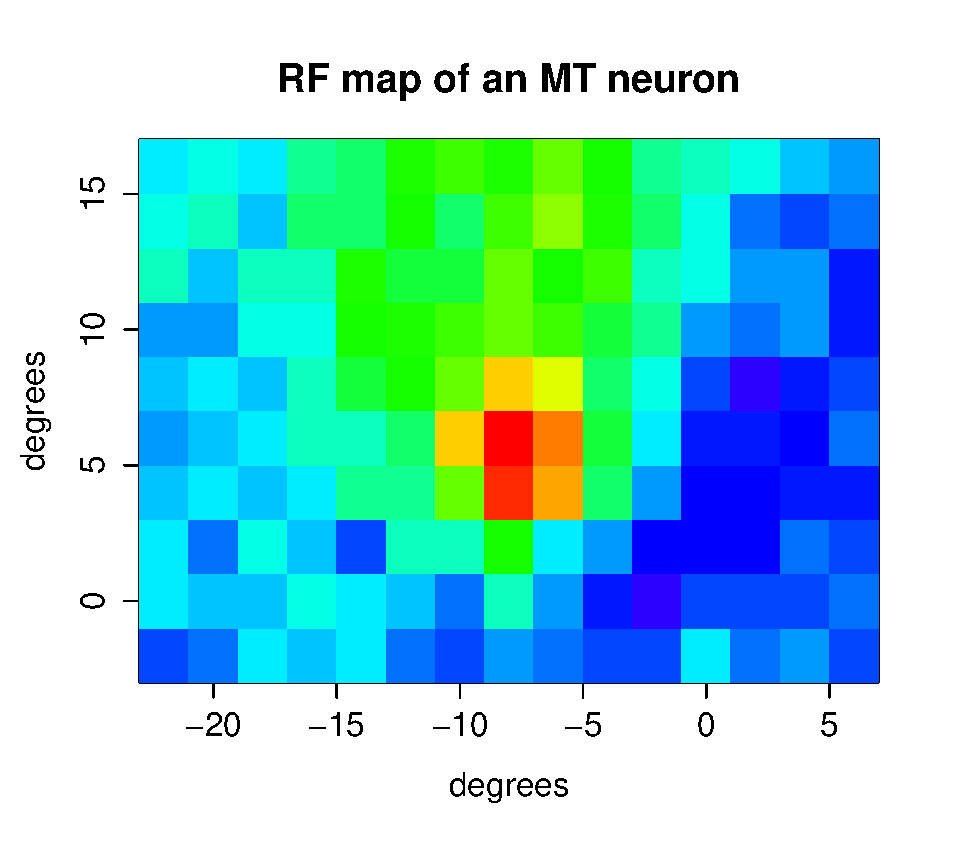
\includegraphics[scale=0.7]{rfmap}
\caption{ The receptive field map showing spike count as a function of location, with red indicating high spike count and blue indicating low.} 
\end{figure}


You will get a tidier figure if you only include stimulus driven spikes, in this case, spikes that occur later than 50ms after the onset of the stimulus.  Why?  This neuron, like most, has a latency period before it will begin to fire spikes.  This neuron's latency is about 50ms.  So if you get spikes that happened later than 45ms then you are pretty sure to be counting all of the relevant spikes and ignoring the irrelevant spikes.  Run the loop above again, using only the relevant spikes by substituting in the below code.

\begin{shortrcode}
>   numspks[ypos, xpos]<- sum(RFmap[ypos, xpos, , ] >45)
\end{shortrcode}


You might add a fixation point as well, to indicate the center of gaze and to see where the receptive field is located with respect to the fovea. You can make the plot full-screen by clicking the \textbf{Zoom} button in your \textbf{Plots} tab. A more publication-ready plotting method is the function \begin{ttfamily}filled.contour\end{ttfamily}, which interpolates and smooths between the sampled points. 
\newline
\newline

\begin{shortrcode}
 filled.contour(x, y, numspks/nTrials, nlevels = 30,
               plot.title = title(main = "RF map of an MT neuron",
                                  xlab = "degrees", ylab = "degrees"),
               # choose colors
               col = rev(rainbow(30,start=0,end=0.7)),
               # add a point
               plot.axes={
                 axis(1); # plot the x-axis
                 axis(2); # plot the y axis
                 # The center of the visual field of the monkey was at (7.5, -7.5)
                 # Let's put a + sign to mark the spot
                 points(0, 0, pch = "+", cex = 2, col = "white", font = 2)}
               )
\end{shortrcode}

\begin{figure}
\centering
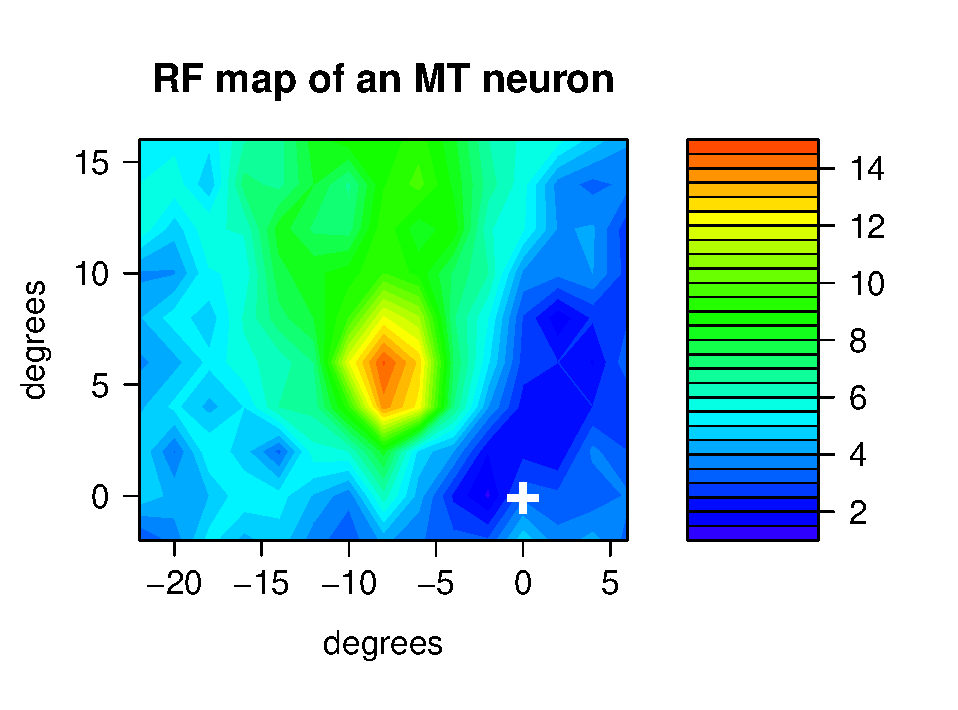
\includegraphics[scale=0.7]{rfmap_45} 
\caption{The RF map counting only spikes occurring $>45$ms post stimulus onset. The white cross indicates the direction of gaze. Spike count values have been smoothed.}
\end{figure}


The script file \verb+plot_RFmap_v2.R+ is a complete algorithm.  Consult it for help, more comments, or run it to check your work.

\section{Exercise 2.  Plot a direction tuning curve}

Many sensory neurons are ``tuned" for a particular feature of a stimulus, meaning that the firing rate changes smoothly as a function of that value.  In MT, many neurons are tuned for the direction and the speed of motion with the highest firing rate for a preferred direction and preferred speed.   We have given you data of 8 MT neurons responding to a range of motion directions and speeds to show their direction and speed tuning. Clear your workspace, then load the data from these neurons.

\begin{shortrcode}
rm(list=ls())

load("../Data/MTneurons8.RData")
print(ls())
\end{shortrcode}   

The data array \begin{ttfamily}spikes\end{ttfamily} contains the responses of all 8 MT neurons to motion in 24 different directions, spaced about the circle in $15^{\circ} $ incremements.  The visual stimulus consisted of random patterns of dots that moved coherently (all had the same direction and speed) in an aperture window centered on each neuron's RF.  Each trial in the experiment consisted of a 200ms motion step in a single direction at one speed.   Inspect the array \begin{ttfamily}spikes\end{ttfamily} to see how the data is organized.

\begin{shortrcode}
dim(spikes)
\end{shortrcode}   

The array \begin{ttfamily}spikes\end{ttfamily} has the dimensions directions (24) by speeds (8) by trials (32) by time (200 milliseconds) by cells (8).   Instead of spike times as before, we now have placed a ``1" into each time bin in which a spike occurred on that trial for a specific stimulus, and bins with no spikes indicated by a 0. The stimuli for each cell were repeated a different number of times, so we have also included the array \begin{ttfamily}nReps\end{ttfamily}, a vector containing the number of repetitions recorded for each cell.  If a cell was recorded for less than 32 trials, we have padded the trials with NaN (stands for "not a number", an indicator that there is no data point there). The vectors \begin{ttfamily}directions\end{ttfamily} and \begin{ttfamily}speeds\end{ttfamily} contain the recorded directions and speeds of motion, and \begin{ttfamily}dates\end{ttfamily} contains the information of when each cell was recorded.


Let's start by applying the skills you learned in Exercise 1 to find the average number of spikes fired for each motion direction from the array \begin{ttfamily}spikes\end{ttfamily} and then plot that value as a function of direction.  The direction values are stored in the vector \begin{ttfamily}directions\end{ttfamily}), and the speed values are stored in the vector \begin{ttfamily}speeds\end{ttfamily}.   

Refer to \verb+plot_tunecurve_v3.R+ for more tips if needed. 

Type

\begin{shortrcode}
nReps[1]
\end{shortrcode}   

to display the number of repeats for each motion direction for neuron 1.  You can see that this cell was recorded for 32 trials at each direction. Let's collect the spikes for only the first cell, and only on the trials that we recorded.  


\begin{shortrcode}
cellnum<-1
spikes_cell<-spikes[,,1:nReps[cellnum],,cellnum]
\end{shortrcode}   


How many spikes did the cell fire on a trial to a specific stimulus? As an example, sum the number of spikes on the first trial to direction \#13 and speed \#4: $15^{\circ}$, $8^{\circ}/$sec:


\begin{shortrcode}
sum(spikes_cell[13,4,1,])
\end{shortrcode}   


You should find that the cell fired 11 spikes in this time window on this trial. To calculate the mean spike count for all directions, we sum over time, then take the mean across trials. We use the function \begin{ttfamily}rowSums\end{ttfamily} to sum across the 4th dimension (time) by telling the function to keep the first three dimensions. We then can use \begin{ttfamily}rowMeans\end{ttfamily} in a similar fashion to take the mean along the 3rd dimension (trials):

\begin{shortrcode}
spikecount_sum<-rowSums(spikes_cell,dims=3)
spikecount_mean<-rowMeans(spikecount_sum,dims=2)
\end{shortrcode}   

You should now have an array \begin{ttfamily}spikecount\_mean\end{ttfamily} with dimensions 24 by 8, containing mean spike count for each combination of direction and speed stimuli presented. To find the direction tuning curve, collapse across speeds by taking the mean along the 2nd dimension, and scale by the amount of time recorded (200ms) to get tuning in units of spikes/second.

\begin{shortrcode}
mean_rates_dir<-rowMeans(spikecount_mean)*(1000/200) 

# Plot the tuning curve
print(
  plot(directions,  mean_rates_dir,
       xlab = 'direction (degrees)', # x label
       ylab = 'Average firing rate (spikes/s)',
#set title
       main = paste('Direction tuning curve'),
#set y axis limits to fit everything
       ylim=c(0,70)
  )
)
\end{shortrcode}   

To add error bars, calculate the standard deviation across trials first. First, make an empty vector to concatenate your standard deviation values for each direction, then add lines indicating error bars to your plot:

\begin{shortrcode}
sddir<-vector()
for (dir in 1:length(directions)){
#c(x,y) combines x and y into a single vector
#sd(x) calculates standard deviation of a vector
  sddir<-c(sddir,sd(spikecount_sum[dir,,]*(1000/200) ))
}

#plot vertical segments of errorbars
segments(directions, mean_rates_dir-sddir,directions, mean_rates_dir+sddir)
#width of top/bottom of errorbars
segwidth = 2
segments(directions- segwidth,mean_rates_dir-sddir,directions+ segwidth,mean_rates_dir-sddir)
segments(directions- segwidth,mean_rates_dir+sddir,directions+ segwidth,mean_rates_dir+sddir)
\end{shortrcode}   

You will generate a figure that looks like this:

\begin{figure}[!ht]
\centering
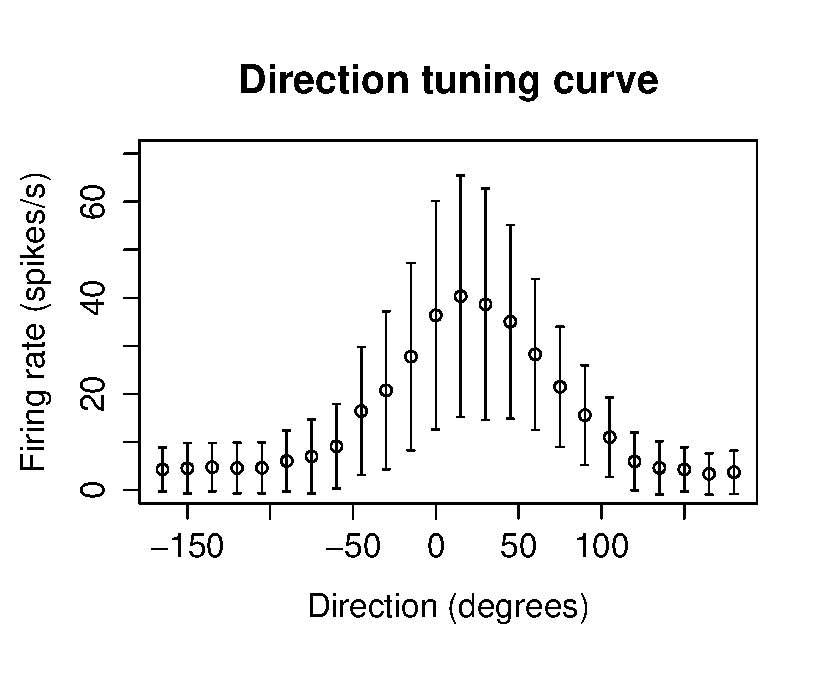
\includegraphics[scale=0.7]{dirtune_wEB} 
\caption{ The firing rate in spikes per second for each motion direction around the circle. Markers indicate the mean over repeats, and errorbars indicate SD. Here we pooled data with different stimulus speeds.} 
\end{figure}
 
We call the direction that elicits the highest firing rate for the cell the ``preferred direction" of this cell.  We can identify this cell's preferred direction by identifying the stimulus eliciting the maximum spike count:

\begin{shortrcode}
maxdir_index<-which(mean_rates_dir==max(mean_rates_dir)
directions[maxdir_index]
\end{shortrcode}   

\textbf{Question:} What is the background firing rate of this cell?  Tip: use spikes occurring at times earlier than 60ms after motion onset. Remember that neurons have a response latency. For the cell you are working with now, the response latency is approximately 70ms. Spikes occurring at earlier times cannot be driven by the motion of the stimulus. Rather, they occur from background network activity. How does the level of background activity affect your ability to detect a motion stimulus from this neuron's spikes? \newline

\textbf{Question:} How large is the difference between the firing rate at the preferred direction and at the opposite direction? 

\section{Exercise 3:  Plot a speed tuning curve and direction-speed tuning}    

This recording also includes data about this cell's responses to speed, so we can calculate the speed tuning in the same way as we calculated direction tuning.  Notice that speed tuning is plotted in $log_2$ units: plotting (and sampling) in log units allows us to understand patterns at the wide range of speeds to which MT neurons respond. 

\begin{shortrcode}
mean_rates_spd<-colMeans(spikecount_mean)*(1000/200)

print(
  plot(log2(speeds),
       mean_rates_spd,
       xlab = 'log2(speed) (degrees per second)', # x label
       ylab = 'Average firing rate (spikes/s)',
       main = paste('Speed tuning curve'),
       ylim=c(0,80)
  )
)

sdspeed<-vector()
for (speed in 1:length(speeds)){
  sdspeed<-c(sdspeed,sd(spikecount_sum[,speed,]*(1000/200) ))
}

#plot vertical segments of errorbars
segments(log2(speeds), mean_rates_spd-sdspeed,log2(speeds), mean_rates_spd+sdspeed)
#width of top/bottom of errorbars
segwidth = 0.02
segments(log2(speeds)-segwidth,mean_rates_spd-sdspeed,log2(speeds)+segwidth,mean_rates_spd-sdspeed)
segments(log2(speeds)-segwidth,mean_rates_spd+sdspeed,log2(speeds)+segwidth,mean_rates_spd+sdspeed)
\end{shortrcode}   

You may notice that the error bars are quite large, so it may seem difficult to distinguish what speed was presented to the cell based on the cell's firing rate. Since cells in MT modulate their firing rates to both direction and speed, try plotting speed tuning at the cell's preferred direction. You can alter this code to also plot direction tuning at a single speed to compare to direction tuning at all directions. 

Here, we use the plot command \begin{ttfamily}points\end{ttfamily} to plot the speed tuning for one direction on the same plot as we previously plotted speed tuning for all directions. The last argument in the \begin{ttfamily}print\end{ttfamily} command functions to change the color.

\begin{shortrcode}
mean_rates_1spd<-as.vector(spikecount_mean[13,])*(1000/200)

print(
  points(log2(speeds),
       mean_rates_1spd,
       xlab = 'log2(speed) (degrees per second)', # x label
       ylab = 'Average firing rate (spikes/s)',
       main = paste('Speed tuning curve'),
       ylim=c(0,80),
       col='red'
  )
)

#get sd again
sd1speed<-vector()
for (speed in 1:length(speeds)){
  sd1speed<-c(sd1speed,sd(spikecount_sum[20,speed,]*(1000/200) ))
}

#plot vertical segments of errorbars
segments(log2(speeds), mean_rates_1spd-sd1speed,log2(speeds), mean_rates_1spd+sd1speed,col='red')
#width of top/bottom of errorbars
segwidth = 0.02
segments(log2(speeds)-segwidth,mean_rates_1spd-sd1speed,log2(speeds)+segwidth,mean_rates_1spd-sd1speed,col='red')
segments(log2(speeds)-segwidth,mean_rates_1spd+sd1speed,log2(speeds)+segwidth,mean_rates_1spd+sd1speed,col='red')
\end{shortrcode}   

\begin{figure}
\centering
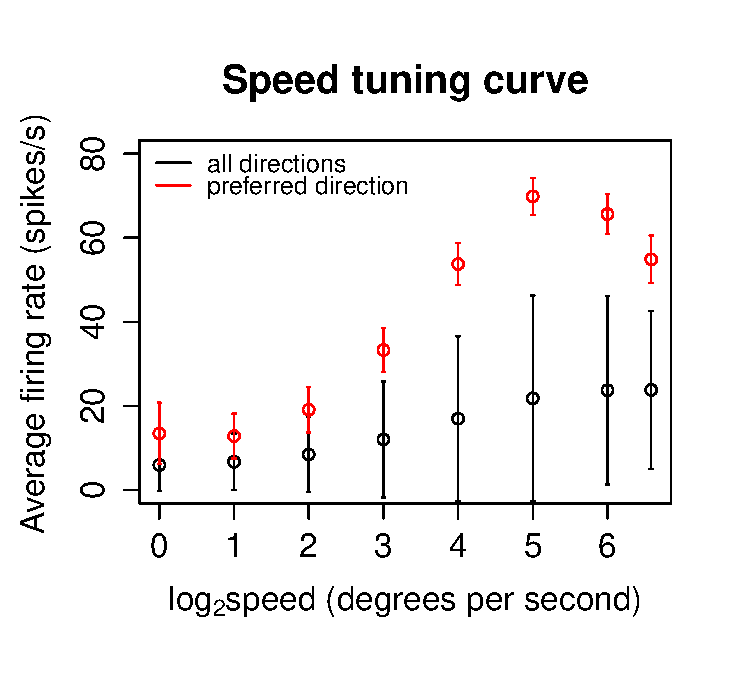
\includegraphics[scale=0.7]{spdtune_log_wEB} 
\caption{Firing changes changes smoothly with speed.  Black circles indicate the direction-averaged rate. Red circles
indicate firing rate for $\theta=15^{\circ}$ }
\end{figure}
 
You can add more speed tuning curves at different directions to this plot to visualize how speed tuning can change as a function of direction. 

We can move one step further by plotting the two-dimensional tuning curve for this cell: how firing rate changes as a function of both direction and speed. One easily visual way to do so is to plot a heat map, as we did with receptive field mapping. We've calibrated the colors so that \textcolor{blue}{blue} indicates low spike counts, and \textcolor{red}{red} indicates high spike counts. 

\begin{shortrcode}   
image(directions,log2(speeds),spikecount_mean, col=rev(rainbow(30,start=0,end=0.7)))
\end{shortrcode}   


\begin{shortrcode}   
filled.contour(directions,log2(speeds),spikecount_mean,nlevels=30,
               plot.title = title(main = 'spike count for an MT neuron',
                                  xlab =  'direction (degrees)',
                                  ylab = 'log(speed) (degrees per second)',),
               col=rev(rainbow(30,start=0,end=0.7))
)
\end{shortrcode} 

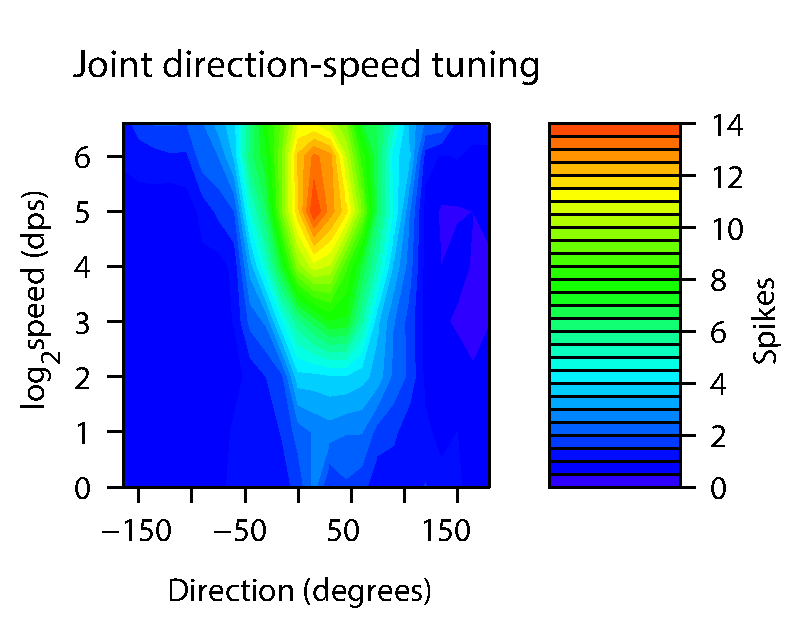
\includegraphics[scale=0.7]{2dtunecurve} 


\section{Exercise 4:  Plot the firing rate as a function of time and direction}   

By summing across time, we're losing a great deal of information that the neuron is communicating by changing its firing rate over time. In this exercise you will be forming a peri--stimulus time histogram (PSTH) to visualize those changes and uncover clues to more complex interactions between neurons. 

\begin{figure}
\centering
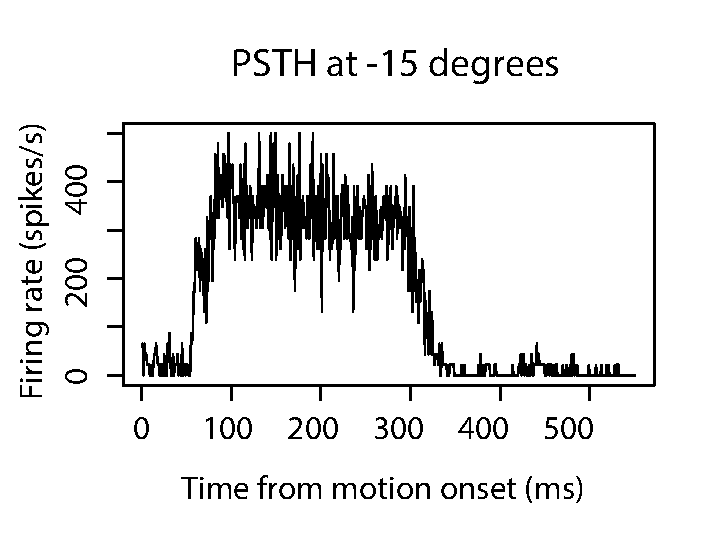
\includegraphics[scale=0.7]{psth1d}
\caption{Average firing rate of an MT neuron over time to motion direction of -15 degrees.}
\end{figure}

The PSTH is the firing rate of the neuron, determined by averaging the response across repeats of the stimulus.  If you compute the PSTH for each direction and plot what you get in direction and time, you'll be making this plot.  In practice, you want to create an array called PSTH that is directions (24) by time (550) (or vice versa) and use the 
\begin{ttfamily}plot\end{ttfamily} command to plot the PSTH for one direction or the 
\begin{ttfamily}image\end{ttfamily} to plot the result for all directions as a 2D color density plot. 
Now load data from another neuron with many repeats to see how direction tuning changes over time.
In this experiment, the stimulus moved for the first 250ms, then stopped moving while we continued to record the neuron's responses for another 300ms. 

If you need to jump ahead or check your work, the script \verb+plot_2Dpsth_v3.R+ for the full code.

First, we'll load the data and make an empty array called PSTH with dimensions 
550 (time) by 24 (directions) to fill in with the mean spike rate for each time bin.

 \begin{shortrcode}
load("../Data/MTneuron_long.RData")
maxTime<-550
nDirs<-length(directions)
PSTH <- array(0, c(maxTime, nDirs))

\end{shortrcode}

The array \begin{ttfamily}spikes\_long\end{ttfamily} contains spikes as before: there is a $1$ in any time 1--ms bin  in which a spike was fired.  You should also have a variable \begin{ttfamily}nReps\_long\end{ttfamily} that indicates the number of repeats for each motion direction. Compute the PSTH, which is the neuron's trial--averaged response as a function of time for each motion direction. 

\begin{shortrcode}

 for (n in 1:nDirs){
#average just over the actual trials for each direction, then multiply by 1000 to get units of spikes per second
PSTH[ ,n] <- rowMeans(mydata[, n, 1:(nReps[n])])*1000 
 }  
\end{shortrcode}

Now, we can display the neuron's time-varying firing rate by plotting the PSTH at the preferred direction. You can prove to yourself using code from earlier that direction \#12 is this neuron's preferred direction.

\begin{shortrcode}

plot(PSTH[,12], 
     type = "l", 			# plot lines instead of points for a cleaner figure
     xlab = 'time from motion onset (ms)', 	# x label
     ylab = 'Average firing rate (spikes/s)',	# y label
     main = paste('PSTH of MT neuron response to ', directions[12], 'degrees') #title
)
\end{shortrcode}

This neuron shows a clear preference for motion over a static stimulus. You can also see that the neuron's firing rate is higher at the beginning of the response, peaking around 100ms.  We call that the ``transient" response, and it quickly decays to a slightly lower firing rate for the rest of the duration of the stimulus: the ``sustained" response. If we plot the PSTH for all directions on the same figure, even more interesting timing dynamics come to light. We'll use \begin{ttfamily}filled.contour\end{ttfamily} again to display those. 

\begin{shortrcode}
print(
  filled.contour(1:maxTime,  directions,  (PSTH), 
    nlevels = 30,    
                    plot.title = title(main = 'PSTH vs direction for an MT neuron',
                     xlab =  'time since motion onset (ms)'),
   	 ylab = 'Direction (degrees)',
    # choose colors
    col = rev(rainbow(28,start=0,end=2/3))
  )
)
\end{shortrcode}

\begin{figure}
\centering
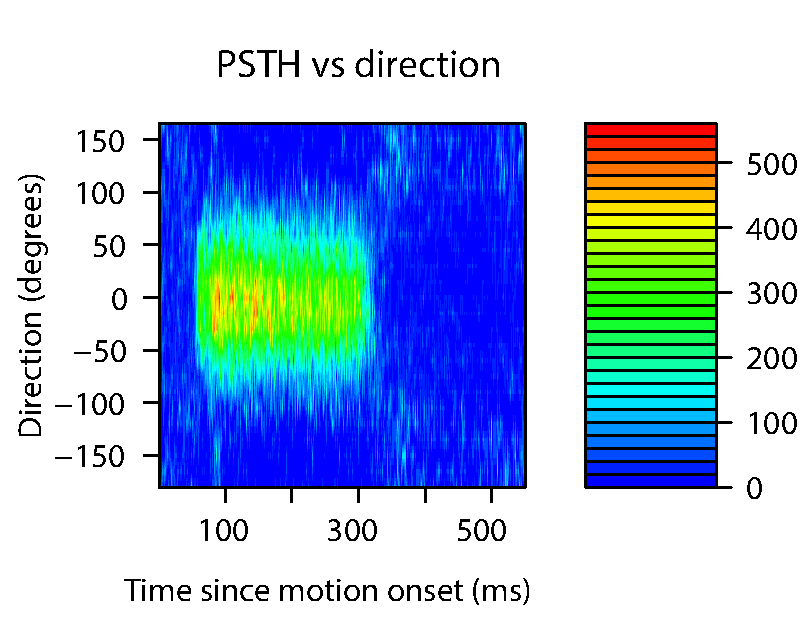
\includegraphics[scale=0.7]{PSTH} 
\caption{Average firing rate over time of an MT neuron.}
\end{figure}
Click the \textbf{Zoom} button at the top of your \textbf{Plots} tab to make this plot full-screen. What features of the cell's response do you see?  Compare the background firing rate (spikes before 50ms) to the firing rate while the stimulus is on.   Try plotting the PSTH for single directions to highlight these firing rate changes. 

Are there any times while the stimulus is moving, or after it stops moving, that the firing rate appears to be lower than the background firing rate? Why might that happen? What effect could that have on perception?

\section{Exercise 5:  Direction and speed tuning over time }   

Let's now return to our other set of neurons modulated by directions and speeds, and apply what we've seen about timing dynamics to see how direction and speed tuning change and interact at different points in the neural response.  
A trick we can use to smooth out some of the variability in spiking behavior is to bin spikes over small time windows. 
We can select specific time bins, sum spikes over those and take the mean across trials. 

To simplify our computations, let's also reshape the \begin{ttfamily}spikes\_cell\end{ttfamily}  array 
to put the time (4th) dimension first, using the \begin{ttfamily}aperm\end{ttfamily} function. 
In this way, we can easily take the mean across trials while keeping the time dimension unaffected. 
A helpful R command to quickly sum spikes in each time bin is \begin{ttfamily}colSums\end{ttfamily}, 
which takes the sum of an array along its first dimension (in this case, time), 
leaving us with an array of total spikes fired for each repetition of each stimulus direction presentation. 
While we're doing this, we can find out the maximum spikes per time bin to use for our plot axis in the next step.


\begin{shortrcode}
binsize<-10
spikes_rot<-aperm(spikes_cell,c(4,1,2,3))
#create this array now so you can fill it during the loop
spikect_binmean<-array(0,c(dim(spikes_rot)[1]-binsize,length(directions),length(speeds)))

for (timebin in 1:(dim(spikes_rot)[1]-binsize)){
  spikect_binsum<-colSums(spikes_rot[timebin:(timebin+binsize),,,],dims=1)
  spikect_binmean[timebin,,]<-rowMeans(spikect_binsum,dims=2)
}
maxsps<-max(spikect_binmean)

\end{shortrcode}

Now we have a variable, \begin{ttfamily}spikect\_binmean\end{ttfamily}, that has the mean spike count in 10--millisecond sliding time windows for each direction and speed. We can cycle through this, plot each time bin using 
\begin{ttfamily}filled.contour\end{ttfamily} heat maps, and see the spike count change over time.  

\textbf{Question:} Does the preferred speed or preferred direction change over time?  
What does this mean for how the brain might ``read out" or interpret the activity of visual neurons to identify the stimulus?

\begin{shortrcode}

#toString to convert numbers to strings
#Sys.sleep(seconds) pauses the calculations and plotting
#You can speed up the animation by changing the increment value in 
#			seq or by reducing the Sys.sleep time
#press the escape (esc) key to break out of the loop and animation

numlevels<-30
for (timebin in seq(1,(dim(spikes_rot)[1]-binsize),1)){
  filled.contour(directions,log2(speeds),spikect_binmean[timebin,,],levels=seq(0,maxsps,(maxsps/numlevels)),
                 plot.title = title(main = paste('spike count from',toString(timebin),'to',toString(timebin+binsize),'ms'),
                                    xlab =  'direction (degrees)',
                                    ylab = 'log(speed) (degrees per second)',),
                 col=rev(rainbow(numlevels,start=0,end=0.7)))
  Sys.sleep(0.1)
}
\end{shortrcode}

Try using different bin sizes.   At what point does it seem like there is no change in the dynamics over time? \newline

\textbf{Question:}  Consider the challenge of trying to read the spikes.  The time scale over which you count spikes will determine what you think the motion direction and speed are when tuning is dynamic.  What are the trade offs between sampling on very short (ms) timescales vs.\ have a longer integration time?  What if you are trying to ``listen" for this neuron in a background of noise where it is harder to resolve individual spikes?  Will that affect will that have on your choice of time bin? 

You can also use the tricks from the PSTH exercise to plot just the time---direction PSTH or the time---speed PSTH to uncover patterns in the data. 

Don't forget that there are 7 more cells in the \begin{ttfamily}spikes\end{ttfamily} variable. You can take a look at any of those by entering 

\begin{shortrcode}
spikes_cell<- spikes[, ,1:nReps[k] , , k] 
\end{shortrcode}

for cell $k$, then running the code in this exercise, to see the variability in different cells' timing dynamics.

\chapter{The statistics of neural responses}~

How reliable are the neuron's responses to repeated stimuli?  If we controlled all of the inputs to the neuron, the answer is that its outputs would be extremely reliable (e.\ g.\ Mainen ZF, Sejnowski TJ (1995) Reliability of spike timing in neocortical neurons.\  Science 268: 1503-1506).  Therefore, the cellular mechanism of generating spikes is not inherently noisy.  However, while recording from a neuron embedded in the brain, the responses to repeated presentations of visual stimuli are variable because we control only a limited number of experimental parameters that can modulate a neuron's input.   In this exercise you will characterize the variability in an MT neuron's response from the experimenter's point of view.  How much of that variability constitutes noise that affects the brain's estimate of motion from that neuron's responses is an open (and interesting) question.    

To get a visual sense of the variability in spiking to repeated motion stimuli, run the script \verb+plot_MTraster_v2.R+ to create a raster plot of the spike times on different trials for this data set.   You may be able to see patterns in the data that you didn't see with the PSTH in the last exercise. 

Type \begin{shortrcode}
speed<-4
\end{shortrcode} (for example) to plot the raster of all directions for the 4th speed in the list of speeds. Each row of a raster plot indicates a spike time on one stimulus presentation with a dot or line.  The rows indicate the neuron's responses on different trials.   Color indicates the different direction values in the same order as directions.  Remember that the motion stimulus begins at time 0 and lasts for 200 ms.   What is the latency of this neuron's response to motion?  Does the latency depend on direction?  What do you notice about the variability of spiking during driven vs.\ spontaneous firing periods?

\begin{figure}
\begin{minipage}{0.55\textwidth}
  \centering
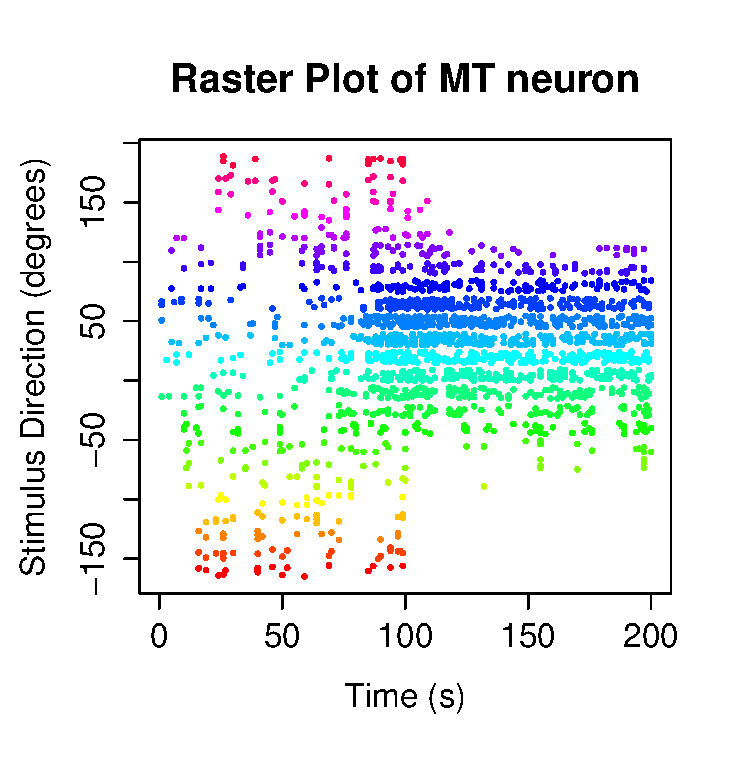
\includegraphics[scale=0.6]{raster}
  
\end{minipage}%
\begin{minipage}{0.55\textwidth}
  \centering
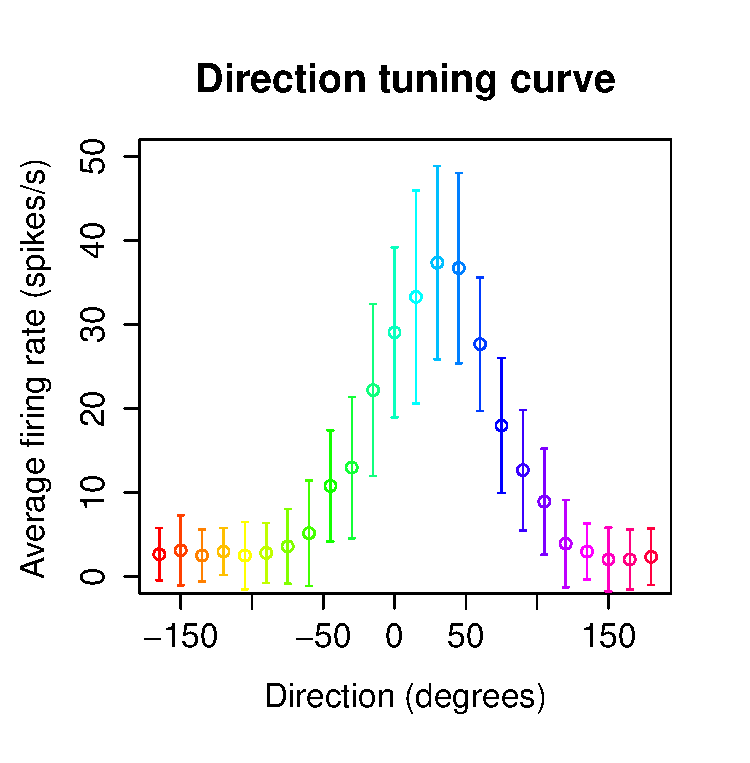
\includegraphics[scale=0.6]{colored_dirtune}
\end{minipage}%
\caption{Left panel: Each dot represents a spike. Each color indicates a different motion direction. Right panel: Mean firing rate, colored to correspond to directions in left panel.}
\end{figure}

The time at which spikes are fired relative to the onset of visual motion varies from trial to trial, as does the number of spikes fired.   Suppose that MT neurons encode motion direction with the number of spikes fired in a certain time window.  In that case, variability in the spike count will create variability in the estimates of motion direction for any downstream decoding of this neuron's responses.  

\section{Exercise 6. Calculate the probability of spiking for a range of directions}~ What is the probability of observing a particular count value in a time window of duration $T$, given the motion direction, $\theta$? i.\ e.\ 
$P_T(n \mid \theta =\theta_i)$.  How does the shape of the distribution change with direction (and thus with the average firing rate)?  Choose the preferred direction and an off-preferred direction and compare the count distributions by making a figure: you can find these directions from the tuning curve plot you made, or the 2D PSTH plot that shows the firing rate change with direction.   Choose a time window of 200 ms from motion onset, and then try other time windows if you have time.  The objective of this exercise is to gain experience in computing a probability distribution and to gain insight about spike count variability.  

A useful R command for measuring the fraction of trials is \begin{ttfamily}hist(array, breaks)\end{ttfamily}, which outputs a histogram, computing the number of data points contained in bins, whose edges are defined by \begin{ttfamily}breaks.hist(array, breaks)\end{ttfamily} returns a structure, and you will want the variable \begin{ttfamily}counts\end{ttfamily} within that structure, which contains the counts within each bin. To access variables within a structure, you use the \$ operator, as shown below. 

\begin{shortrcode}
#set up variables again to make sure
load("../Data/MTneurons8.RData")
cellnum<-1
spikes_cell<-spikes[,,1:nReps[cellnum],,cellnum]
spikecount_sum<-rowSums(spikes_cell,dims=3)
spikehist<-array(0,c(length(directions),length(speeds),(max(spikecount_sum)+1)))

#bins to separate spike count (including 0 spikes)
bin_edges<-seq(0,max(spikecount_sum)+1,1)-0.5

for (d in 1:length(directions)){
  for (s in 1:length(speeds)){
    #hist: defining bin edges to bin spike counts
    #hist gives a list of components and plots histogram
    #we extract "counts" component by following hist command with $counts
    #suppress plot by plot=FALSE
    spikehist[d,s,]<-hist(spikecount_sum[d,s,],bin_edges,plot=FALSE)$counts
  }
}
\end{shortrcode}


At this point, you can compute the probability of the count given the motion direction in your time window, i.\ e.\ 
 $P_{T}(n \mid \theta)$.  The probability is like a frequency or a fraction --- how many times did you observe a count of $n$, out of all the repetitions?  

\begin{shortrcode}
PnGstim<-spikehist/nReps[cellnum]
\end{shortrcode}


Make a 1D plot of $P(n \mid \theta=\theta_{i})$ (probability of observing counts of different values given that the motion was in a particular direction, $\theta_i$ and a particular speed, $v_i$.  

\begin{shortrcode}
theta<-13
v<-6
print(plot(1:dim(PnGstim)[3],PnGstim[theta,v,],
      type = "l", # plot lines
      xlab = 'Spike count',
      ylab = expression(paste('P(n| ',theta,')')),ylim=c(0,0.5))
)
\end{shortrcode}


Do this for the preferred direction and speed, which elicits the highest firing rate, and an off-preferred direction with a lower firing rate.  Use color or line type to denote the 2 different directions as we did before.  How does the likelihood of observing a particular count value change as a function of direction? To really visualize this you could step through all the directions, but you will have a crowded figure unless you just choose a few!  
\begin{figure}
\centering
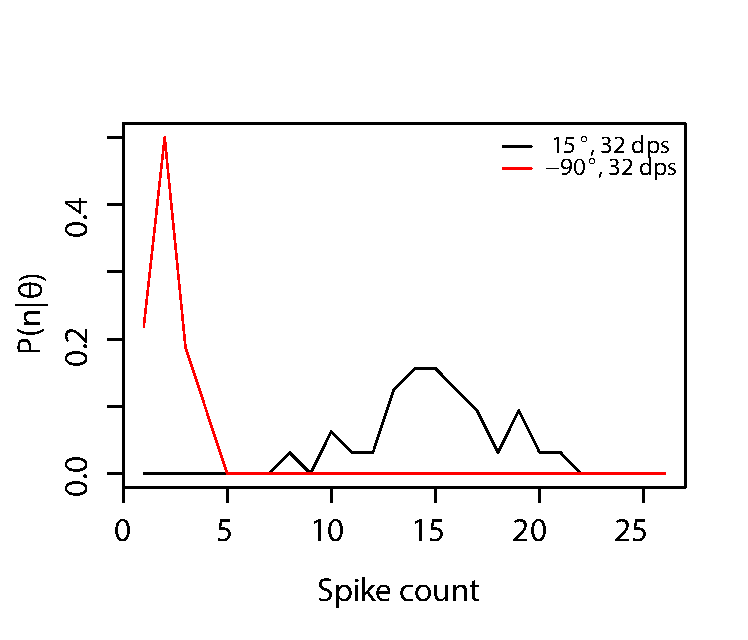
\includegraphics[scale=0.7]{conditionalcount} 
\caption{Distributions of the probability of spike count given two different stimulus directions.}
\end{figure}

Is the mapping between count and direction unique?  These distributions are the answer to the question, ``Given the direction, what is the most likely spike count".  The problem that the brain faces is better phrased, ``Given the spike count, what is the most likely direction?"  That distribution is $P(\theta \mid n)$. We can generate this probability distribution by taking our array \begin{ttfamily}spikehist\end{ttfamily} for each spike count $n$ and dividing by the number of times any stimulus presentation resulted in that spike count. 

If the cell did not fire any spikes in the repetitions recorded for a specific stimulus, we will be dividing by zero.  A safeguard against this is to add epsilon (accessed by \begin{ttfamily} .Machine\$double.eps \end{ttfamily}) to the denominator, which is the minimum value that can be represented by your machine. Epsilon is typically $ 2.2 \mathrm{x} 10^{-16} $, so even though it is infinitesimally small, it avoids the issue of dividing by zero but does not affect your calculations. 

\begin{shortrcode}

for (n in 1:(max(spikecount_sum)+1)){
PstimGn[,,n]<-spikehist[,,n]/(sum(spikehist[,,n])+.Machine$double.eps)
}
\end{shortrcode}

Inspect your probability distributions by stepping through each spike count and plotting a heat map of $P(\{\theta, v\}\mid n)$. 

\begin{shortrcode}
for (n in 1:(max(spikecount_sum)+1)){
  
  
  filled.contour(directions,log2(speeds),PstimGn[,,n],levels=seq(0,0.2,0.2/30),
                 plot.title = title(main = paste('stimulus probability from',toString(n-1),'spikes')),
                                    xlab =  'direction (degrees)',
                                    ylab = 'log(speed) (degrees per second)',
                 col=rev(rainbow(30,start=0,end=0.7))
                 )

Sys.sleep(0.1)
}
\end{shortrcode}

How is this affected by different spike count binning? Try changing \begin{ttfamily}bin\_edges \end{ttfamily}argument in the
 
\begin{shortrcode}
spikehist[d,s,]<-hist(spikecount_sum[d,s,],bin_edges,plot=false)$counts
\end{shortrcode}

 command a few steps above. Consider that a stimulus that elicits 10 spikes on average would also have a standard deviation (SD)  of $\pm \sqrt 10 = 3$ spikes. What might happen with bin edges of [0,2,4,7,10,14,18,22,27,32], so that bin size increases proportional to the SD?

A legitimate complaint at this point would be that the brain can use a large population of neurons to generate estimates, so we may want to evaluate our uncertainty of estimating the stimulus when we use multiple cells. Use the below code to repeat the process above for all cells in the spikes array.

\begin{shortrcode}

numcells<-8
spikecount_sum_allcells<-array(0,c(length(directions),length(speeds),max(nReps),numcells))
spikecount_mean_allcells<-array(0,c(length(directions),length(speeds),numcells))

for (cellnum in 1:numcells){
  spikes_cell<-spikes[,,1:nReps[cellnum],,cellnum]
  spikecount_sum_allcells[,,1:nReps[cellnum],cellnum]<-rowSums(spikes_cell,dims=3)
  spikecount_mean_allcells[,,cellnum]<-rowMeans(spikecount_sum_allcells[,,1:nReps[cellnum],cellnum],dims=2)
}

bin_edges<-seq(0,max(spikecount_sum_allcells)+1,1)-0.5
spikehist_allcells<-array(0,c(length(directions),length(speeds),length(bin_edges)-1,numcells))
PstimGn_allcells<-array(0,c(length(directions),length(speeds),length(bin_edges)-1,numcells))

for (cellnum in 1:numcells){
  #calculate histograms
  for (d in 1:length(directions)){
    for (s in 1:length(speeds)){
      spikehist_allcells[d,s,,cellnum]<-hist(spikecount_sum_allcells[d,s,1:nReps[cellnum],cellnum],bin_edges,plot=FALSE)$counts
    }
  }
  #normalize for each spike count bin
  for (n in 1:dim(spikehist_allcells)[3]){
    PstimGn_allcells[,,n,cellnum]<-spikehist_allcells[,,n,cellnum]/(sum(spikehist_allcells[,,n,cellnum])+.Machine$double.eps)
  }
  Sys.sleep(1)
}
\end{shortrcode}

What are the relative probabilities for the estimate of a stimulus given the response from all cells? Try direction index 16, speed index 4 as an example.  Step through cells to combine the $P( \{ \theta,v\} \mid n)$ distributions for the (rounded) mean spike count for each cell. The cell-averaged distribution is $P(\mathrm{stimulus_{estimated}} \mid \mathrm{stimulus_{actual}})$. 
You can also wrap this code in \begin{ttfamily}for\end{ttfamily}loops to cycle through the direction and speed indices and watch how the variance of the estimate changes. 

\textbf{Question: } How much is the estimate variance affected by the preferred directions and speeds of cells we have sampled?  Which neurons are the most and least informative about the stimulus?  What does this suggest about integration of spikes across a pool of neurons in the brain?

\begin{shortrcode}

#for each stimulus value, make empty stimprob_estim to generate distribution
    stimprob_estim<-array(0,c(length(directions),length(speeds)))
       for (cellnum in 1:numcells){
         spikect_estim<-round(spikecount_mean_allcells[dirindex,spdindex,cellnum])
         if (sum(PstimGn_allcells[,,spct_est,cellnum])>0){
           stimprob_estim<-stimprob_estim+PstimGn_allcells[,,spikect_estim,cellnum]
          }
        }
      
stimprob_estim<- stimprob_estim/sum(stimprob_estim) #normalization

filled.contour(directions,log2(speeds),stimprob_estim,levels=
				seq(0,max(stimprob_estim),max(stimprob_estim)/30),
                     plot.title = title(main = 'stimulus probability'),
                     xlab =  'direction (degrees)',
                     ylab = 'log(speed) (degrees per second)',
                     col=rev(rainbow(30,start=0,end=0.7))
      )

  Sys.sleep(1)

\end{shortrcode}

How do these estimates change depending on how much of the response you use? 
Go back to your array \begin{ttfamily}spikecount\_sum\end{ttfamily} and run through this code again while only using the transient response, for example. Is there much difference in your ability to estimate the stimulus 
as time elapses and more spikes are available?

\end{document}
